\label{ml}
\namedsection{Machine Learning}{Playle}

\note{What even is machine learning?}
Machine learning is a technique that takes some observations about a system in addition to a value of interest \todo{Maybe s/value of interest/output/}, builds a model around these parameters and uses this model to create predictions about the value of interest for the system. There are typically three categories of machine learning algorithm: classification, where the value of interest is in a finite set of classes; regression, where the value of interest is continuous...... \todo{}

In order to detect exercise, a classifying machine learning algorithm will be most suitable, with the classes being types of activity observed.

\subsection{Considered Issues}

%%%%%%%%%%%%%%%%%%%%%%%%%%%%%%%
%%% CURSE OF DIMENSIONALITY %%%
%%%%%%%%%%%%%%%%%%%%%%%%%%%%%%%
One of the frequently encountered problems is the curse of dimensionality \cite{bellman1957dynamic}. Having a high number of dimensions, often as a result of having a large number of inputs into a machine learning algorithm, can create the problem whereby the amount of instances required to sufficiently train the model increases as the amount of training of the model must have instances such that the input feature space must be explored sufficiently. \cite{oommen2008objective}. Further to this effect, the time and space complexity of many machine learning algorithms are functions of the feature space's dimensionality. However, existing work has demonstrated that the curse of dimensionality is not necessarily applicable to time-series data as the nature of such data explores the feature space on the condition that the signal-to-noise ratio is sufficiently high \cite{bernecker2011quality}.

\note{How exactly does the machine learning algorithm work? Reference papers that describe these methods.}

\note{What experiments were conducted in order to determine machine learning feasibility?}
\subsection{Initial Feasibility Assessment}
In order to initially determine the feasibility of applying machine learning for detecting exercise, a simple experiment was conducted with a single subject. The intent of the experiment was to implement a similar machine learning algorithm as is described in \cite{kwapisz2011activity} to ensure understanding of the problem at hand.

The collection device used came in the form of a Sony Z3 mobile phone, providing kinematic sensors, of which the gyroscope, measuring the angular velocity, was used. The subject had the collection device attached to their foot while they performed activities including a foot rotation exercise; walking on a flat surface; and walking up and down stairs. Additionally, noise was collected by moving the collection device in random directions. The collection device sampled data at 200Hz on each axis, so for the purpose of assessing feasibility, this value was carried through into machine learning, using a window size of 200 samples for a classification over 1 second intervals.

Data for each activity was collected separately to ensure classification could be performed without having to note exact timings of activities. Some examples of the data collected in these activities are shown in figure \ref{fig:first-data}, where the periodic nature of all the activities (with the exception of noise), can be seen clearly. \todo{Discuss this data more?}

This data was run through a series of tools to build a model, as described in section \ref{sec:tools-produced}. Initial evaluation of the performance was conducted using 10-fold cross-validation. The confusion matrix for a simple naive Bayes classifier is shown in table \ref{tab:first-confusion}.

The results for this initial experiment were promising, clearly indicating that the model was able to distinguish between the activities.

\begin{table}[]
	\centering
	\caption{Feasibility Assessment Confusion Matrix \label{tab:first-confusion}}
	\begin{tabular}{|cccc|ll|}
		\hline
		\multicolumn{4}{|c|}{Classified As}   &          &                        \\
		Exercise & Noise & Stairs & Walking &          &                        \\
		\hline
		62       & 0     & 0      & 0       & Exercise & \multirow{4}{*}{Class} \\
		2        & 15    & 1      & 0       & Noise    &                        \\
		3        & 0     & 10     & 3       & Stairs   &                        \\
		1        & 0     & 1      & 7       & Walking  &                       \\
		\hline
	\end{tabular}
\end{table}


\begin{figure}
	\centering
	\subfigure[Exercise]{\label{fig:first-exercise}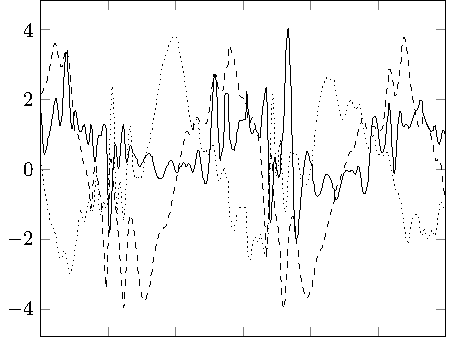
\includegraphics[width=70mm]{figures/first-exercise.pdf}}
	\subfigure[Noise]{\label{fig:first-noise}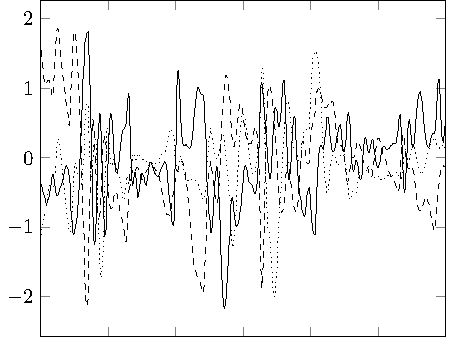
\includegraphics[width=70mm]{figures/first-noise.pdf}}
	\subfigure[Stairs]{\label{fig:first-stairs}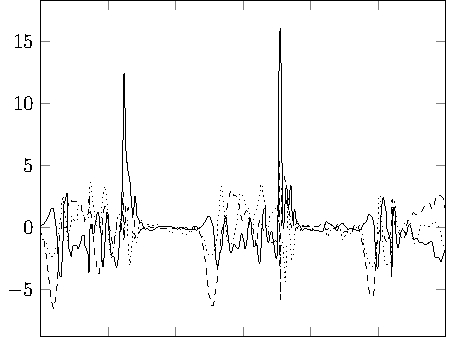
\includegraphics[width=70mm]{figures/first-stairs.pdf}}
	\subfigure[Walking]{\label{fig:first-walking}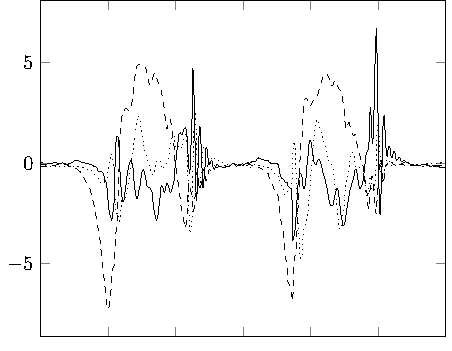
\includegraphics[width=70mm]{figures/first-walking.pdf}}
	\caption{Feasibility Assessment Data \label{fig:first-data}}
\end{figure}

\subsection{Tools Produced \label{sec:tools-produced}}
\note{Tools produced}

\note{Why did we use 3 classes rather than just 2?}
The number of classes to classify was considered, as a variable parameter for the classifier. A classifier with the 2 classes \textit{exercise} \todo{Maybe s/exercise/activity/} and \textit{not exercise}, would only allow for binary classification. Depending on the classifier behaviour and the nature of the exercise in question, it may be the case that when the window of classification lies between 2 exercises, the window could be classified as either class. This unpredictable behaviour would prevent further analysis of the subject's exercise beyond how much time exercise has been detected for. \todo{Add figure}. However, by splitting the \textit{exercise} class into 2 distinct classes, such that every exercise performed will always be composed of these parts, it allows 3 classes to be used with the classifier. Such a change would allow counting of distinct exercises, by ensuring that one type of \textit{exercise} class is followed by the other type of \textit{exercise} class. This would allow the number of exercises to be counted, as well as the amount of time exercised. Further to this, the additional information may allow for heuristics to increase accuracy should the classifier ``bounce''. \todo{More on this in heuristics...} Other numbers of classes were also considered, such as some number of classes for the exercise, along with a class for each likely type of non-exercise activity. \todo{and this idea was rejected because...}

\note{What classification algorithms were trialled? What kind of results were achieved with these. Explain and discuss the workings of each algorithm / type of algorithm.}

\subsection{Multilayer Perceptrons}
A Multilayer Perceptron (MLP) is a type Neural Network, where the nodes, or perceptrons, are organised in layers. Each node accepts some number of inputs with some weight. These summation of these weighted inputs are computed and applied to some activation function, the result of which is the output of the node (equation \ref{eq:perceptron}).

\begin{equation}
\label{eq:perceptron}
\text{Output } o = activation\bigg(\sum_{i=1}^{d}{x_iw_i}\bigg) 
\end{equation}

Each perceptron affectively defines a plane in $d$-dimensional space. Instances on either side of this plane can then be classed, allowing a single perceptron to act as a simple classifier. By combining multiple perceptrons in a layer, it is possible to build up these planes in order to create more complex classifier made of these linear classifiers. The addition of layers, using previous layers are inputs allows a more complex classifier still by allowing the importance of these sub-classifiers to vary with the inputs. MLPs with enough inputs and layers can therefore replicate any function \cite{baum1988capabilities}.

\note{Finish/tidy this and wrap in figure}
\begin{tikzpicture}[shorten >=1pt,node distance=1.3cm and 3cm,on grid,auto,initial text={}] 
\node[state,initial] (i1) {$i_1$};
\node[state,initial] (i2) [below=of i1] {$i_2$}; 
\node[state,initial] (in) [below=of i2] {$i_n$}; 

\node[state] (h11) [right=of i1] {$h_{1,1}$};
\node[state] (h12) [below=of h11] {$h_{1,2}$}; 
\node[state] (h1a) [below=of h12] {$h_{1,a}$}; 

\node[state] (hb1) [right=of h11] {$h_{b,1}$};
\node[state] (hb2) [below=of hb1] {$h_{b,2}$}; 
\node[state] (hba) [below=of hb2] {$h_{b,a}$}; 

\node[state] (o) [right=of hb2] {$o$};
\path[->] 
(i1) edge node {} (h11) (i2) edge node {} (h11)
(i1) edge node {} (h12) (i2) edge node {} (h12)
(i1) edge node {} (h1a) (i2) edge node {} (h1a)
(in) edge node {} (h11) (h11) edge node {} (hb1)
(in) edge node {} (h12) (h11) edge node {} (hb2)
(in) edge node {} (h1a) (h11) edge node {} (hba)
(h12) edge node {} (hb1) (h1a) edge node {} (hb1)
(h12) edge node {} (hb2) (h1a) edge node {} (hb2)
(h12) edge node {} (hba) (h1a) edge node {} (hba)

(hb1) edge node {} (o)
(hb2) edge node {} (o)
(hba) edge node {} (o)
;
\end{tikzpicture}

\subsection{Radial Basis Function Networks}

\subsection{Instance-Based Learning}
Instance-based learning is a type of machine learning algorithm that postpones model creation until an output for a problem instance is required. Some number of labelled instances are stored in memory, and these are used to label problem instances.

Instance-based learning is advantageous over other machine learning methods in that adapting the model with new instances is trivial. This makes it attractive for simple systems where some adaptation of the model is required.

As a number of labelled instanced must be kept in memory in order to compute the model, instance-based learning methods can require large amounts of memory to classify. Additionally, any problem instances must be compared against each labelled instanced that is to be used for the model, meaning that time complexity for classification of any problem instance is linear in the number of labelled instances. This can present significant challenges when the size of the training data set become large with respect to the underlying device.

An example of instance-based learning is the k-nearest neighbours algorithm where any problem instance is compared to the k-nearest labelled instances. The class that the problem instance is most similar to is then given this classification. \todo{Reword}

\note{What issues were faced as a result of implementing a machine learning algorithm on a constrained system? How were these problems overcome? \cite{anguita2012human}}
Each machine learning algorithm comes with its own memory-processing-accuracy trade-off, 

\note{What tools were used in order to assist with the machine learning?}
Machine learning was assisted with Weka... \todo{}

\note{As a result of the user study, how did the results change? Note observed results due to the user study.}

\note{What metrics were used to measure machine learning classifier performance?}

\note{What parameters are there and how did they affect the accuracy of the system?}